\documentclass[conference,letterpaper]{IEEEtran}

\ifCLASSINFOpdf
  \usepackage[pdftex]{graphicx}
  \graphicspath{{images/}{figures/}}
  \DeclareGraphicsExtensions{.pdf,.jpeg,.png}
\else
  \usepackage[dvips]{graphicx}
  \graphicspath{{figures/}}
  \DeclareGraphicsExtensions{.eps}
\fi
\newcommand{\subparagraph}{}

\newtheorem{definition}{Definition}
\newtheorem{property}{Property}
\newtheorem{theorem}{Theorem}

\usepackage{amsmath}
\usepackage{color}
\usepackage{xcolor}
\usepackage{colortbl}
\usepackage{listings}
\usepackage{multirow}
\usepackage{mdframed}
\usepackage{url}
\usepackage[subsubsection]{algorithm}
\usepackage{algpseudocode}
\usepackage{lipsum}

\definecolor{LightCyan}{rgb}{0.88,1,1}
\definecolor{BluishGray}{RGB}{226,227,231}
\definecolor{LightGray}{gray}{0.95}
\definecolor{Gray}{gray}{0.85}
\usepackage{amsthm}
%\usepackage{enumitem}
\usepackage[numbers,sort&compress]{natbib}

\theoremstyle{plain}

\theoremstyle{definition}
\newtheorem{defn}{Definition}
\newcommand{\ti}{\textit}
\newcommand{\tb}{\textbf}

\lstset{
language=Ada,                % choose the language of the code
basicstyle=\footnotesize,       % the size of the fonts that are used for the code
%numbers=left,                   % where to put the line-numbers
%numberstyle=\footnotesize,      % the size of the fonts that are used for the line-numbers
%stepnumber=1,                   % the step between two line-numbers. If it is 1 each line will be numbered
%numbersep=5pt,                  % how far the line-numbers are from the code
backgroundcolor=\color{white},  % choose the background color. You must add \usepackage{color}
showspaces=false,               % show spaces adding particular underscores
showstringspaces=false,         % underline spaces within strings
showtabs=false,                 % show tabs within strings adding particular underscores
%frame=single,           % adds a frame around the code
tabsize=2,          % sets default tabsize to 2 spaces
captionpos=b,           % sets the caption-position to bottom
breaklines=true,        % sets automatic line breaking
breakatwhitespace=false,    % sets if automatic breaks should only happen at whitespace
escapeinside={\%*}{*)},          % if you want to add a comment within your code
numbers=right,
numbersep=-10pt,
numberstyle=\tiny,
}

\algrenewcommand{\alglinenumber}[1]{\scriptsize#1:}

\makeatletter
\renewcommand{\ALG@beginalgorithmic}{\scriptsize}
%\renewcommand{\thealgorithm}{\arabic{section}.\arabic{algorithm}}
%\newcommand{\darkalglinenocolor}{%
%   \alglinenumber[1]{\color{black}\footnotesize#1:}}
%%  \setcolor{ALG@color}{\color{black}}}
\makeatother

\begin{document}

\title{Model-driven development and traditional coding - Mind the gap!}

\author{
	\IEEEauthorblockN{Van Cam Pham, Shuai Li, Ansgar Radermacher, Sébastien Gérard, Chokri Mraidha, Rémi Schnekenburger}
	\IEEEauthorblockA{CEA, Address\\
		Email: \{first-name\}.\{last-name\}cea.fr}
}

\maketitle

\begin{abstract}
%Model-Driven Engineering (MDE) is a development paradigm that brings the benefits of increased automation to the software development cycle.
%The MDE community tries to promote MDE adoption by pushing models written in diagram-based languages, supported by extensive tooling.
%While there is increasing evidence that MDE facilitates the design of complex software, its level of acceptance by software developers is still low.
%On one hand, rather than use diagram-based languages, most programmers prefer to work with their favorite text-based languages (e.g. Java and C++)
%and integrated development environment.
%On the other hand, software architects are among the early adopters and promoters of diagram-based languages.
%They consider such languages to be much more suitable for describing architectures compared to textual languages.
%Synchronizing manually written artifacts in either type of language is not simple and is often very time-consuming and error prone unless it is supported
%by automated methods and tools.

%To solve this issue, we propose a methodological pattern for model-code synchronization supported by corresponding tooling. 
%The solution tackles a fundamental problem of round-trip engineering: synchronization between concurrently evolving artifacts. 
%On one side we have the architecture model maintained by the software architects, while on the other, we have code written by programmers.
%Applying our approach for the development of an actual runtime system, we show that both parties involved, software architects and programmers, can efficiently collaborate while continuing to work in their favorite development environment.
\end{abstract}


%\begin{IEEEkeywords}
%Key words
%\end{IEEEkeywords}

%\thispagestyle{plain}
%\pagestyle{plain}

%TODO introduce notion of viewpoint consistency and say that it is an important part of what we propose and why we propose it
%TODO reinforce notion of collaboration between software architects and programmers, that is a motivation of our work
\section{Introduction}
\label{sec:introduction}

% What is MDE and how are models seen by the MDE community who creates a gap between modeling and coding
Internet of Things \cite{Li2015} raises the complexity of embedded systems today rapidly. 
Model-Driven Engineering (MDE) is recognized as an efficient means to deal with the complexity.
MDE \cite{selic_what_2012} promotes abstraction and automation. 
The latter often relies on chaining transformations from source models at high level abstraction to target models and finally to code. 
Those two techniques are identified as model to model (M2M) and model to code (M2C) transformations.
%Traditionally, the MDE community draws a sharp distinction between development
%using a diagram-based language (commonly called a modeling language in the MODELS \cite{models_conf} community)
%and development using a textual language (i.e. a programming language or code). 
Among modeling languages, the Unified Modeling Language (UML) is most widely used. 
UML and its diagrams are much more useful to design such systems than text-based languages. 
Especially, in embedded system domains such as vehicle controlling, UML State Machines \cite{Cruz-Lemus2005} are used as a powerful means to describe the dynamic behavior of such complex systems.

%Proponents of MDE have argued that adopting model-centric approaches
%would benefit software developers due to its many advantages
%\cite{selic_what_2012}, especially for development of complex systems.
%They encourage the greater use of model-driven development,
%by, among other initiatives, providing diagram-based languages
%supported by appropriate tools \cite{gerard_once_2015}
%such as automated code generation.

% Problem: perceived difference between diagram-based language and textual language
%In industrial practice, there is still significant reticence to adopt a
%fully model-centric approach \cite{hutchinson_model-driven_2011, selic_what_2012}.

%This is all the more true
%for models that are described in diagrams \cite{brown_position_2015}.
Ideally, a full model-centric approach is preferred by the MDE community due to its advantages \cite{selic_what_2012}. However, in industrial practice, there is significant reticence \cite{Hutchinson:2011:MEP:1985793.1985882} to adopt it. 
The reticence is due in part to
the perceived gap \cite{brown_position_2015} between diagram-based languages
and textual languages.
On one hand, programmers prefer to
use the more familiar textual programming language. 
On the other hand, software architects, working at higher levels
of abstraction, tend to favor the use of models, and therefore
prefer graphical languages for describing the architecture of
the system (see Fig. \ref{fig:inconsistency}).

The survey described in \cite{hutchinson_model-driven_2014,Forward2008} polled stakeholders in companies
who use MDE approaches. 
The survey reveals that UML is the prominent and dominating language. 
85\% of the respondents used UML for various purposes, especially problem understanding and automation such as code generation (88,2\%). 
It notes that 70\% of the respondents primarily work
with models, but still require manually-written code to be integrated.
Furthermore, 35\% of
the respondents answered that they spend a lot of time and effort synchronizing
model and code. The need of synchronization is critically required by systems today. 
Besides the synchronization aspect, efficiency of code generated from models is a concern for the respondents. 

%Yet, still in another survey \cite{Forward2008}, the authors compare code-centric and model-centric approaches by asking the participants, who mostly come from Canada, United States and other countries such as United Kingdom, France, Indian, Australia and Singapore, questions related to different activities in software development such as fixing a bug, creating efficient software and a system as quickly as possible. 
%The results shows that most activities tend to be easier in a model-centric approach but many participants believe that a code-centric approach is much easier a model-centric approach.
%This confirms the importance of automatically keeping model and code synchronized.
      

The code modified by programmers and the model are then inconsistent. 
Round-trip engineering (RTE) \cite{Hettel2008} achieves synchronization between related artifacts
that may evolve concurrently by incrementally updating each artifact
to reflect editions made in the other artifacts.
RTE enables actors (software architect and programmers) to freely move between different representations \cite{Sendall} and stay efficient with their favorite working environment. 

Even, if the code is not intended to be modified by programmers, RTE is still helpful in the state-of-the-art MDE practice, e.g. debugging generated code. Some code generators generate fully operational code. The debugging support helps developers trace bugs in the generated code back to precise model elements. 

% Problem: even in MDD, as described by the MDE community, code is not entirely moved out
%Even in teams who embrace a model-driven approach,
%the gap between model and code is not bridged seamlessly.

The back-and-forth switching between diagram-based and textual languages, as well as
between model and code,
%along with the effort necessary for artifacts synchronization,
has hindered the adoption of MDE in industrial practice.
To solve this issue, we believe that the sharp distinction between model and code must be blurred.
We feel that a collaborative solution must be offered to
different categories of developers (e.g. architects, programmers),
who use different development practices.
%The solution must not impose a choice between a diagram-based language and a textual language.


\begin{figure}
	\centering
	\includegraphics[trim={4.5cm 6.6cm 5cm 3cm},clip, width=0.8\columnwidth]{figures/inconsistency}
	\caption{Concurrent modifications made to different artifacts}
	\label{fig:inconsistency}
\end{figure}

Collaboration between developers producing different types of artifacts, in different languages,
using different tools,
raises the issue of artifact synchronization.
This is a well-known concern with round-trip engineering \cite{sendall_taming_2004}.
%Namely, round-trip engineering requires the ability to maintain consistency
%between multiple concurrently evolving software artifacts \cite{sendall_taming_2004}.
It is related to traditional software engineering disciplines
such as forward
and reverse engineering \cite{chikofsky_reverse_1990}.



Usually, a direct synchronizing between the architecture model and the code is hard because of the large abstraction gap. The synchronization is therefore decoupled into several synchronization steps of artifacts participating in one of the transformation phases of the chain. Hence, the whole synchronization is achieved if these steps do. 

\subsection{Research method}
The research is realized by an iterative method depicted in Fig. \ref{fig:researchmethod}.
We started by studying the literature related to MDE and approaches to integrating MDE into industrial practice. 
We are interested in approaches for developing embedded systems using synchronization of model and generated code, which is critical as previously discussed.
Specifically, we found that, (1) current approaches and tools do not support synchronization of concurrent modifications made to model and code. Furthermore, (2) the synchronization is, for UML community, only supported for available concepts of UML class diagrams while the behavior model such as UML State Machine (USM) is not supported.
The reason is that there is no trivial mapping between mainstream programming languages such as C++ and Java, and the behavior model.

However, USM plays an important role in modeling and designing reactive, real-time, embedded systems.
Hence, the lack of synchronization support for USMs harms enterprises to adopt UML as a development language.
%It is how our motivation is established.


It is common in MDE that code is generated, from either USMs or component models, by using templates.
When models or templates change, code needs to be changed accordingly.
However, when these artifacts are concurrently modified, for some reasons, making these consistent again are challenging. 
Some approaches using specialized comments such as \ti{@generated} and \ti{@non generated} to specify which code areas should be untouched or modified, respectively.
By this way, when model elements and code change, code areas (user-modified code) marked by \ti{@non generated} are preserved. 
It means that changes made to models or templates are not propagated to some code areas. 
This may lead to the dead code problem, in which the user-modified code is not used in the new generated code (see \ref{subsec:sync-template} for more details).
Hence, we realize (3) the problem of models, code, and template co-evolution, which is not solved by existing approaches.

Once these related problems are identified, we then focus on defining and resolving the problems by proposing different approaches, whose goal to gain the acceptance of MDE by the enterprises.
The development and evaluation of the solutions are then conducted.
We iteratively evaluate by going to results of evaluation, compare with other approaches, and check whether the solutions can be improved to get better results.
%Once

\begin{figure}[b]
	\centering
	\includegraphics[trim={1.0cm 0.2cm 2.0cm 7.3cm},clip, width=1.04\columnwidth]{figures/researchmethod}
	\caption{Research method}
	\label{fig:researchmethod}
\end{figure}

\subsection{Major topics}
\label{subsec:majors}
To sum up, the thesis can be divided into two related major parts as followings:
\begin{itemize}
	\item \tb{Artifact synchronization}: As previously discussed, this is critical for step-by-step integrating MDE into current software development practices and collaborating these with MDE methodologies. Particularly, synchronization of artifacts is realized by means of incremental model-to-model and model-to-text transformations. Architecture models are often at a higher level abstraction than low level implementation code. Mappings from the architecture are usually not one-to-one. This raises the difficulty in mapping code-side elements back to architecture model-side elements. The existing synchronizations (state of the art) mainly focus on static parts while the dynamics are missing.
	
	\item \tb{Improving code generation solutions and towards synchronization for UML State Machine}: UML State Machines are widely used for reactive, real-time and embedded systems. However, the synchronization between UML State Machine and generated code is not supported by any existing approaches, even though it is critical. 
	Furthermore, on the one hand, the OMG seeks to raise the usefulness of UML State Machine by providing more modeling concepts supporting software architects for modeling and designing complex systems. 
	On the other hand, the support of existing generation approaches, over the years of research and development, is still limited to simple cases, especially when considering concurrency, pseudo state and event support. 
	
	\item \tb{Co-evolution of models, code, and generation templates}.  
	
	%\item \tb{Model-code co-debugging (MCCD)}:	Debugging is one of the most important activities in software development to find and fix bugs. 
	%In MDE, when having bugs in generated code, it is difficult to locate the code statements or the model elements, which have the bugs. 
	%MCCD enables modelers/developers to set breakpoints on model elements/code statements, respectively, and the breakpoints are also set on the associated code elements/model elements.
	%Thus, MCCD helps seamlessly collaborate model and code in debugging.
	%Current tools and approaches \cite{moka} support the model execution and debugging, especially for UML Activity and State Machine Diagrams, using Java/fUML as underlying action language.
	%However, model-code co-debugging 	 
\end{itemize}

\begin{comment}
In reality, UML State Machine might be used for different use-cases, either with RTE or not. 
We consider the second topic in different use-cases. Fig. \ref{fig:smapproaches} shows three cases. 
There are trade-offs between these. In the use-case (a), code generators can generate efficient code from state machines with full features (this is detailed in this report).
The case (b) (see \ref{subsec:usm2code}) only supports a small sub-set of modeling features and trades a reversible mapping with a memory overhead. 
The case (c) is a harmonization of the other two but restricts developers to a domain specific language (DSL). 

\begin{figure}
	\centering
	\includegraphics[trim={5.4cm 8.1cm 11.6cm 4.2cm},clip, width=0.8\columnwidth]{figures/smapproaches}
	\caption{Different usages of UML State Machine code generators and RTE: (a) state machines are generated to code and modifications only made to the state machines; (b) code generated from state machines is modified and synchronized directly with the state machines; and (c) generated code is modified indirectly via a text-based domain specific language (DSL).}
	\label{fig:smapproaches}
\end{figure}


\subsection{Problem statement}
\begin{itemize}
	\item Architecture models are often at higher level abstraction than low level implementation code. Mappings from the architecture are usually not one-to-one. This raises the difficulty in mapping code-side elements back to architecture model-side elements. The existing synchronizations mainly focus on static parts while the dynamics are missing.
	
	\item While UML State Machine are a powerful means to modeling the logical behavior of complex systems, the support for generating code from state machines and the efficiency of the generated code are limited to non-concurrency with issues such as memory consumption and processing speed. 
\end{itemize}
\end{comment}

\subsection{Objective}
The transformation from architecture models to code directly involves chaining model-to-model and model-to-text transformations. Therefore, to synchronize the architecture models and code, the following objectives need to be met:
\begin{itemize}
	\item A generic methodology, which synchronizes two different system artifacts (model and code). This method is based on incremental model transformation and synchronization. It will be used in different specific synchronization cases developed in the thesis deployment.
	
	\item A specific synchronization between UML State Machine with full features and code. %This will gain the usage of MDE in software development today. 
	Therefore, one task is needed to 
	%seamlessly make the behavior of the code generated from UML State Machine complied with the semantics specified by the Precise Semantics of UML State Machine (PSSM) \cite{OMG2015}. 
	%To do it, the objective of this part is to 
	provide a complete generation solution, especially considering the concurrency support for real-time systems. From the generation solution, a specific synchronization methodology combined with the generic one as above is also desired.  
	
	\item Synchronization of and making concurrently modified models, code, and templates consistent again.    
\end{itemize}

The final goal is to provide a common framework with many facilities for collaborating MDE developers and programmers so effectively that the acceptance of MDE in practice can be gained.

\subsection{Contributions}
The contributions of this report are the followings:
\begin{itemize}	
	\item An extensible generic methodology, which synchronize two different system artifacts (model and code). 
	
	%\item A complete generation solution from UML State Machine to code with respect to the Precise Semantics State Machine (PSSM). 
	
	\item A specific methodology for the synchronization of UML State Machine and code. 
	
	%\item A method for synchronization based on incremental model transformations, which prevent one artifact from begin overwritten when propagating changes from the other artifact.
	
	\item Brief presentation of ongoing works around model-code synchronization which are not detailed in this report.
	   
\end{itemize}

\begin{comment}
\subsection{Global vision of the thesis progress}
Fig. \ref{fig:progress} shows the thesis global vision. 
The complexity of complex systems are dealt by the abstraction of MDE, whose core technologies are model transformation, code generation and reverse engineering (see Section \ref{sec:processes} for definitions). 
These core technologies are the state-of-the-art of MDE. 
In order to synchronize different artifacts of systems, MDE researchers introduce incremental transformatio  

\begin{figure}
	\centering
	\includegraphics[trim={0.8cm 4.5cm 1cm 5.6cm},clip, width=\columnwidth]{figures/progress}
	\caption{Thesis progress global vision}
	\label{fig:progress}
\end{figure}
\end{comment}

\subsection{Structure of the report}
The remaining of this report is structured as followings: Section \ref{sec:processes} presents a generic pattern for artifact synchronization in case of concurrent modifications made to model and code. Section \ref{sec:approach} describes a round-trip engineering from UML State Machine (a subset) to code and back. Section \ref{sec:ongoing-future} presents some ongoing works including an approach for round-trip engineering from USMs with full features and C++ code for reactive systems, an approach for co-evolution of concurrently modified models, code, and templates, and a verification of semantic-conformance of generated code runtime execution. Section \ref{sec:other} sketches other works which are not detailed in this report.

\begin{comment}
\subsection{Decoupling of the synchronization of artifacts}
\begin{figure}
	\centering
	\includegraphics[trim={2.5cm 8.5cm 2cm 6cm},clip, width=\columnwidth]{figures/decouple}
	\caption{Concurrent modifications made to different artifacts}
	\label{fig:decouple}
\end{figure}



The work presented in this paper is motivated by the open-source Papyrus-RT \cite{cea_papyrus-rt_2016}
runtime system which was developed in collaboration by companies A, B, and C.
These companies are contributors to the MDE eco-system.
The architecture of this system follows an object-oriented paradigm,
and it was initially implemented as a C++ project with about 15,000 lines of code.
This project
encountered the problem of collaboration
between MDE developers and programmers working in the traditional manner.

% Announce contribution here
In this paper, we propose to use automated model-code synchronization as a means of
bridging the gap between models edited by software architects, and code written by programmers.
Our approach is based on the following contributions, described in detail later in this paper:

\begin{enumerate}
  \item A generic model-code synchronization methodological pattern to solve
  the problem of collaboration between different types of developers,
  when model and code co-evolve. This contribution is based on the following requirement and proposition:
  \begin{itemize}
    \item Requirement: the availability of a generic IDE with functionalities necessary for model-code synchronization.
    The functionalities are not dependent of a particular approach or technology. The required IDE will be described
    in this paper.
    \item Proposition: Processes to use the IDE to synchronize model and code based on several defined scenarios, which correspond to common
    development practices.
  \end{itemize}
  \item An Eclipse-based implementation of the approach for synchronization between UML models and corresponding C++ code.
  \item Experience on applying the proposed solution for the development of a real-world example.
\end{enumerate}

Contrary to traditional solutions, we generalize our work by considering
the case where the model is not only
used for architectural design, but also for
full implementation.
The tooling of our solution
focuses on the Unified Modeling Language (UML),
because it is a very widely used software architecture description language \cite{malavolta_what_2013}.
We want to
synchronize models specified in a diagram-based language like UML with code in a popular textual programming language like C++
(used by 4.4 million \cite{kazakova_infographic:_2016} developers worldwide).

% Announce plan here
The rest of the paper is organized as follows. Section \ref{sec:use-case} defines
the actors (roles) we consider in our work and the use-cases of the generic
IDE for our model-code synchronization approach.
In Section \ref{sec:processes}, we propose processes for synchronizing model and code, in
several scenarios.
A possible implementation of our solution, based on Eclipse technologies, is proposed in Section \ref{sec:implementation}.
The approach is evaluated in Section \ref{sec:experiments} through simulations
and the case-study of Papyrus-RT runtime.
Section \ref{sec:related_works}
relates our work to existing research and industrial approaches.
Finally, in Section \ref{sec:conclusion} we conclude with some perspectives.


\end{comment}
% Say that the gap is too big, imposing only model-based development to companies
% is not viable and has been tried before (failure)
% See case of accor (ancestor of Papyrus)
%TODO
%Topics to consider:
%
%- RTE model/code
%  * Cam's stuffs
%  * Acceleo for architecture/body RTE
%  * Aspect Oriented-based Software Synchronization in Automatic Measurement Systems
%- Model-model synchronization ---> Basically justify our stuffs by saying we use model sync as a mean, and we have a generic pattern, where you just plug other people's model sync techniques. Also same format during sync, so easier to use, especially in case of conflicts.
%  * Google search model synchronization
%  * Tracing evolution changes of software artifacts through model synchronization
%  * Towards automatic model synchronization from model transformations ----> They use ATL. Restricted to a technology. But their artifacts are related by model transformation, which is the case for us too (code must ben generated from model). Human intervention not allowed? They use differentiating of states, while we listen to change events. I.e. Class1 becomes Class2 we can detect this, while they will detect Class1 added, Class2 deleted. Also they always sync two models in two forms while we propose to sync, while having an image so we can use one form. Furthermore they don't handle well reflectable changes target side, i.e. I change the name of a class target side, I can't get it to sync source side? Also they only consider model sync, not the social aspect (this is not bs since we define actors). We use a synchronization artifact in the format the the dev wants to use.
%  * From model transformation to incremental bidirectional model synchronization
%  * Incremental model synchronization with triple graph grammars
%  * Model synchronization at work: keeping SysML and AUTOSAR models consistent
%  * Concurrent Model Synchronization with Conflict Resolution Based on Triple Graph Grammars
%  * Framework-Specific Modeling Languages with Round-Trip Engineering
%- Using viewpoints and synchronizing them: Use viewpoints to represent different aspect of the system. In our case it means architecture in UML viewpoint, and body in C++ viewpoint. The for example verify that composite structure viewpoint is valid according to the class definition viewpoint. Or verify that architecture viewpoints satisfy the requirements viewpoint. I guess this might be similar to model-model synchronization, except several viewpoints can represent the same model.
%  X ViewPoint-oriented software development by distributed graph transformation: towards a basis for living with inconsistencies
%  * A Viewpoint Model for Cooperative Building of an Ontology
%  X Change Management in Multi-Viewpoint System Using ASP
%  X ViewPoint Oriented Software Development, Anthony Finkelstein, Jeff Kramer, -->  Michael Goedicke <---
%  * VIEWPOINTS: A FRAMEWORK FOR INTEGRATING MULTIPLE PERSPECTIVES IN SYSTEM DEVELOPMENT, http://www.worldscientific.com/doi/abs/10.1142/S0218194092000038
%  * ViewPoint oriented software development: Methods and viewpoints in requirements engineering
%  * ViewPoint-Oriented Software Development: Tool Support for Integrating Multiple Perspectives by Distributed Graph Transformation
%  * Early aspects: a model for aspect-oriented requirements engineering
%  * Agent Oriented Software Engineering with INGENIAS
%- Graphical vs textual
%  * Google search graphical textual programming, graphical programming, textual programming, visual programming
%  * === graphical vs textual ===
%  X Scaling up visual programming languages 
%  X Lack of Keyboard Support Cripples Block-Based Programming
%  X Visual Programming Languages and the Empirical Evidence For and Against
%  X Blocks Versus Text: Ongoing Lessons from Bootstrap
%  X End-User Experiences of Visual and Textual Programming Environments for Arduino
%  X Are visual programming languages better? The role of imagery in program comprehension
%  X Comparing the comprehensibility of textual and graphical programs
%  X Why looking isn't always seeing: readership skills and graphical programming: different interpretation of same visual and textual program
%  * === end ===
%  * === Integrating graphical with textual ===
%  X Heterogeneous visual languages-integrating visual and textual programming - integrating visual with textual
%  X Unifying Textual and Visual: A Theoretical Account of the Visual Perception of Programming Languages
%    "This work suggests that the gap between textual and graphical languages is narrow, and that all kind of programming languages should rely on the capability of the human visual system."
%  * LIVE-Integrating visual and textual programming paradigms
%  * Languages and tools for the graphical and textual system independent programming of programmable logic controllers
%  * Visual language as a mean of communication in the field of information technology 
%  * === end ===
%  * === Some graphical languages
%  * Blocks and Beyond workshop http://cs.wellesley.edu/~blocks-and-beyond/schedule.html
%  * 2nd Workshop on Graphical Modeling Language Development http://www.dsmforum.org/events/GMLD13/
%  * Comparing the comprehensibility of textual and graphical programs
%  * Prograph: a step towards liberating programming from textual conditioning
%  * ALF
%  * The CODE 2.0 graphical parallel programming language
%  * Simulink, LabVIEW
%  * Visual programming languages: A survey M Boshernitsan, MS Downes - 2004 - Citeseer
%  * Arduino
%  * === end ===
%- Software maintenance
%  X Mental models and software maintenance
%  X Program comprehension during software maintenance and evolution
%- (Stakeholders collaboration)
%  * Collaboration in Software Engineering: A Roadmap
%  * Collaboration Tools for Global Software Engineering
%
%Big themes:
%- Our technical work ==>
%  * Synchronization and co-evolution: model-code, model-model, viewpoints
%- We want to let each developer use what he wants ==>
%  * Comprehension: visual vs textual, software maintenance based on program comprehension
%  * Integrating visual and textual: integrating both
%
%The paragraphs breakdown:
%§4: Visual vs textual, which is better? For comprehension? (transition: we argue code is a viewpoint and so we compare it with diagram-based viewpoint)
%§3: Viewpoints synchronization (transition: several viewpoints for a model)
%§5: Visual AND textual (transition: but like us, some work think visual and textual can co-exist, so each dev can use the best that suits his/her comprehension [shit under software maintenance topic])
%§1: Model-code RTE tools
%§2: Model sync research works (transition: model sync is generalization of model-code RTE)

\section{Related Work}
\label{sec:related_works}

Our work is motivated by the desire to reduce the gap between
model and code, between diagram-based languages and textual languages.
We use automation-supported model-code synchronization as a means to achieve this goal.
In the following sections, we compare our propositions to related works recorded in the literature.

\subsection{Comparison of diagram-based and textual languages}

Diagram-based languages, also called graphical languages, are a subset of visual languages,.
A number of efforts were undertaken that compared textual languages and visual languages.

Many works \cite{schanzer_blocks_2015, petre_why_1995}
discuss the pros and cons of visual languages, compared
to textual languages, in various contexts. Others \cite{brown_position_2015}
discuss what limits 
the adoption of visual languages.

Contrary to these works, we do not strictly oppose textual languages to visual languages like
diagram-based languages.
Instead, we prefer to blur the boundaries between them.
The idea that visual languages can co-exist with textual languages
has been noted by other authors.
%Others suggest that the gap between visual languages and textual languages is not as huge
%as it is perceived by both the MDE and software engineering communities.

In \cite{conversy_unifying_2014} the authors argue
that the gap between textual and visual languages is narrow.
They propose a framework to represent code in a visual language
to improve comprehension of the code.

In \cite{erwig_heterogeneous_1995} the authors
propose a generic framework to use both visual and textual languages at the same time.
The visual artifacts are translated to textual code. Much importance
is given to the human factor, i.e. the framework can be customized based on developer preferences.

In domains such as requirements engineering,
tools, such as IBM Rational Doors \cite{ibm_doors_2016}
and Visure Requirements \cite{visure_visure_2016},
are conscious of the importance of supporting requirements written
traditionally in plain text by developers.
These tools allow the transformation of requirements written
in a textual human language to use-cases and structured requirements.

However, none of these systems are intended to support full implementation of a system. Generally, one of the artifact
is only used to assist comprehension. There is no need for synchronization between artifacts because
the transformation only proceeds in one direction.

Our argument that, in order to be more efficient, developers should not be forced to choose between
a diagram-based or textual language, is directly related to software comprehension.
Works \cite{von_mayrhauser_program_1995}
that emphasize the role of software comprehension, for
efficient software maintenance and evolution, date back to as far as the late eighties/early nineties.
In our work we consider specifically both software architects and programmers.
The former generally foster diagram-based languages
for architecture description and comprehension.
The latter prefer textual languages since they are deemed much more expressive
for specifying fine-grained algorithms, for example.

\subsection{Artifact synchronization}

Our work is also closely related to synchronization of different artifacts used for development.
In the following paragraphs, our model-code synchronization approach is compared to works
on model-code round-trip engineering,
viewpoint synchronization,
and model synchronization.

\paragraph{Round-trip engineering of model and code}

% RTE tools

Several commercial and open-source tools \cite{EA, ibm_rational_2016, Magicdraw, umlgen} support round-trip engineering between UML models and code.
Systematic reviews of some of these tools are available in \cite{Cutting2015}.
%Support for Java round-trip is prominent in most tools.
%Other languages such as C++ are only available in a few tools \cite{ibm_rational_2016, umlgen, Magicdraw}.
%Our methodological pattern does not focus on a particular programming language
%or a particular modeling language. Furthermore, the current implementation of our approach is dedicated
%to UML and C++, which is less supported by tools than Java.
Usually these tools only support architectural elements on the model-side.
The model cannot be used for full implementation and
dependencies derived from
method bodies are not considered during the round-trip. In our work, we assume that
the model can be used for full implementation. Furthermore, our implementation analyzes
C++ method bodies not only to reverse them to UML, but also to derive dependencies in the UML model.
Some tools \cite{EA} only allow
one of the artifacts, model or code, to be edited at a certain time.
There is then no problem of synchronizing model and code since there are no concurrent changes, which limits their applicability.
Finally, some tools \cite{umlgen} do not support a real incremental reverse or code generation;
instead, they treat change (e.g. renaming) as deletion followed by addition.

% RTE restriction
Some round-trip engineering techniques restrict the development artifact to avoid
synchronization problems.
Partial round-trip engineering and protected regions are introduced in \cite{czarnecki_multi-level_2006}.
Such techniques aim to preserve code editions which cannot be propagated to models.
This approach separates the code regions that are generated from models
from regions which are allowed to be edited by developers.
In contrast to our work,
this form of round-trip engineering is unidirectional and does not support iterative development \cite{Jorges2013}.
Furthermore we do not restrict editions on model and code.

%TODO low-level
%The authors in \cite{angyal_synchronizing_2008} propose a syntactic synchronization technique for domain-specific modeling languages (DSML) and code. 
%The approach uses an Abstract Syntax Tree (AST) metal-model to model source. Changes in code detected by using an algorithm proposed  in \cite{Chawathe:1996:CDH:235968.233366} to compare the AST instance of the current code with the last synchronized one are merged to the instance of DSML. 
%However, an AST is very low level and it is not clear to have mappings from DSML instances to AST instances. 
%Furthermore, although there is an example for illustrating the technique, a systematic evaluation of the approach is not presented to show its scalability.

\paragraph{Viewpoint synchronization}

% Viewpoint
Both models and code can be considered simply as different viewpoints
of the same system. Viewpoints enable the partitioning of the model of a system into several representations. 
Synchronization between viewpoints is crucial to maintain their consistency.

In \cite{eramo_change_2008} the authors improve the modeling of relationships and constraints between
elements in different viewpoints in order to better guarantee the consistency of viewpoints.
In \cite{goedicke_viewpoint-oriented_2000} the authors argue that inconsistencies will exist
in systems developed with different actors, using different viewpoints. They suggest that tools
must be able to tolerate inconsistencies. A distributed graph transformation is proposed to deal with the problem of formalizing the integration of multiple viewpoints in software development.
Their work focuses on requirements engineering.
In contrast, our approach targets specifically both model and code.
Code is not usually considered in viewpoint synchronization because code is deemed to be too fine-grained.
Furthermore, our approach does not require explicit modeling
of relationships between model and code elements.

\paragraph{Model synchronization}

Viewpoints synchronization is generalized by model synchronization for which there is
an abundance of techniques presented in the literature. Model synchronization aims
to maintain consistency between a source model and a target model. 

Many model synchronization techniques require the explicit mapping of source model and target model.
The authors in \cite{Paesschen2005} propose an injective mapping of elements in the source model to
the target model. The mapping can be used for synchronization.
Techniques and technologies, such as Triple Graph Grammar (TGG) \cite{giese_incremental_2006},
and QVT-Relation \cite{Omg2008},
allow synchronization between source and target elements that have non-injective mappings.
The authors in \cite{Hermann2012} formalize TGG for synchronization of models that are concurrently edited.
All of these techniques require a mapping model to connect the source and target models
with typed traceability links, which need to be persisted in a model store \cite{Bergmann2011}.
This means that editing one model requires the presence of the other.
Our model-code synchronization approach does not require a mapping model and an artifact may be edited
independently of the presence of the other corresponding artifact.

Other techniques \cite{foster_combinators_2007}
are based on bi-directional transformations, which comprise a forward transformation of
source to target model, and a backward transformation of target to source model.
Bi-directional transformations provides a novel mechanism for synchronization.
Indeed, some works \cite{Matsuda2015} derive a backward transformation based on forward
transformation.
However, such works do not offer any means to synchronize models that are concurrently edited.

A few approaches derive model synchronization from model transformation while allowing concurrent editions
of both source and target models.
In \cite{xiong_towards_2007} the authors propose to automatically derive
model synchronization of a source and a target model related by an ATL \cite{eclipse_foundation_eclipse_2016}
model transformation.
The synchronization is based on differentiating source and target model states.
But, reflectable addition of an element in the target model is not well handled according to \cite{xiong_towards_2007}.
Our approach is generic and does not depend on a specific technology. Furthermore, in our implementation
we propose to use modification events rather than state differences for incremental
transformations, necessary for synchronization.

~

As a final note, we argue that our methodological pattern is generic. Therefore many synchronization
techniques found in the literature can be integrated into our approach, such as, for example,
the \texttt{Synchronize Model} or \texttt{Reverse Code} use-cases of
the proposed generic IDE.
Finally, our solution targets collaboration between software architects and programmers who wish to use
diagram-based languages or textual languages. Therefore we propose to use a synchronization artifact
in the preferred language of the developer, rather than directly synchronizing artifacts in different languages.

\section{Preliminary definition}
\label{sec:use-case}

In this section we define the actors who will use our model-code synchronization approach to collaborate during development.
%Then we define the main capabilities, as use-cases, expected from a generic IDE used by these actors.
Some basic concepts related to the actors and use-cases are also defined in this section.

\subsection{Collaborating actors and development artifacts}

%In this paper we propose a methodological model-code synchronization pattern for collaboration between software
%architects and programmers.
For the sake of generality, we postulate that the architect and programmer are actors with starkly opposite development practices.
This allows the approach to be used even in cases where model
and code can both be used for the full implementation of a system,
rather than just architectural design for the former,
and code implementation for the latter.
First, we introduce the concepts of \textit{development artifact} and \textit{baseline artifact}.

\begin{definition}[Development artifact]
A development artifact is a artifact, as defined in \cite{omg_software_2008},
that can be used for the full implementation of the system.
\end{definition}

%For example a system can be entirely implemented as code.
%Implementation code is a development artifact, so may model.
%It is then not only documentation of specification
%but part of the implementation.
%For example a model can be used for implementation by generating code from the model, and compiling the code without the need to edit or complete the code.
In our work, we assume that model and code are both development artifacts.
A development artifact may be the baseline artifact, defined in this paper as follows:

\begin{definition}[Baseline artifact]
A baseline artifact is one which may be edited manually.
All other artifacts are produced from the baseline artifact
through some process, and only through a process. Manual edition
of artifacts other than the baseline artifact is forbidden.
\end{definition}

Two primary actors, called \textit{model-driven developer}
and \textit{code-driven developer}, are introduced.
%The main difference between them
%is what they consider as the baseline artifact.

\begin{definition}[Model-driven developer]
A model-driven developer is an actor in a software development process
for whom the baseline artifact is the model.
\end{definition}

%In other words, for the model-driven developer only the model should be edited manually. 
The code must always be produced from the model automatically
by some process that guarantees that the code is consistent with the model.
A software architect is a kind of the model-driven developer
who edits the model to specify the architecture of the system.
%An architect presumes that the reference for the architecture
%of the system should be specified as a model.

\begin{definition}[Code-driven developer]
Code-driven developer is an actor in a software development process
for whom the code is the baseline artifact.
\end{definition}

A programmer is a specialization of the code-driven developer.
Indeed, programmers may modify the code, such as editing method bodies.
%The code is then the main reference for the implementation of methods.

\begin{comment}
\subsection{Main use-cases of IDE for collaboration between developers}
\label{sec:use-cases_ide}

In this section we propose a generic IDE with the main
use-cases that represent functionalities
required by our model-code synchronization approach.
%Figure \ref{fig:use-case} shows a UML use-case diagram of the IDE
%and associations to the actors.

%\begin{comment}
\begin{figure}
\centering
\includegraphics[width=\columnwidth]{figures/use-case}
\caption{Use-cases of IDE for model/code edition and synchronization}
\label{fig:use-case}
\end{figure}
%\end{comment}

%\begin{comment}
There are some use-cases for manual edition of artifacts. The \texttt{Edit Artifact} use-case
implies that the IDE must have some tool to let the developer manually edit an artifact.
The \texttt{Edit Model} and \texttt{Edit Code} use-cases are specializations of the \texttt{Edit Artifact}
use-case where the artifact is the model or code.

There are also some use-cases related to the synchronization of artifacts. The \texttt{Synchronize Artifact} use-case
is the synchronization of two artifacts by: (1) comparing them, (2) updating each artifact with editions made
in the related artifact, and (3) reconciling conflicts when appropriate. The \texttt{Synchronize Model} and \texttt{Synchronize Code}
use-cases are specializations where, respectively, the model or the code are the artifacts being synchronized.

The \texttt{Generate Code} use-case is related to forward engineering.
It is the production of code in a
programming language from a model.
The developer can either use \texttt{Generate Code (Batch)} or \texttt{Generate Code (Incremental)}.
%\end{comment}

\begin{definition}[Batch code generation \cite{Giese2006}]
Batch code generation is a process of generating code
from a model, from scratch.
Any existing code is overwritten by the newly generated code.
\end{definition}

Incremental code generation is a specialization of incremental model transformation, which
is defined in \cite{Giese2006} as model transformation that
does not generate the whole target model from scratch but only updates the target model by
propagating editions made in the source model.

%\texttt{Incremental code generation (ICG)} \ti{$gen_{inc}$ is a process of taking as input a changed model m and an existing executable code to make the code synchronized with the changed model: $gen_{inc}(m, c) = c'$. Non-conflicted changes at the code side are kept intact the synchronization. ICG is also defined as a process of taking model changes ch and an existing code c: $gen_{inc}(ch, c) = c'$}.

%Derived from the definition of incremental model transformation, 
Incremental code generation
is defined in this paper as follows:

\begin{definition}[Incremental code generation]
In-cremental code generation is the process
of taking as input an edited model, and existing code, and then updating the code by propagating
editions in the model to the code.
\end{definition}

%\begin{comment}
Finally, the \texttt{Reverse Code} use-case is related to reverse engineering.
\texttt{Reverse Code} is the production of a model, in a modeling language, from code, written in a programming language.
The developer can either use \texttt{Reverse Code (Batch)} or \texttt{Reverse Code (Incremental)}, which are defined in this paper as follows:
%\end{comment}

\begin{definition}[Batch reverse engineering]
Batch reverse engineering is a process of producing a model from code, from scratch.
The existing model is overwritten by the newly produced model.
\end{definition}

\begin{definition}[Incremental reverse engineering]
Incremental reverse engineering is the process of taking as
input a edited code, and an existing model, and then updating the model by propagating
editions in the code to the model.
\end{definition}

%For readability, in this paper we will sometimes designate batch and incremental as modes
%of code generation/reverse; e.g. we say that we generate code in batch mode from a model.

%The use-cases are generic. They do not depend
%on any particular approach or tool. Therefore the software developers
%can choose the approach or tool that suits better his/her
%development preferences best.

In the next section, the use-cases of the IDE are integrated into
some processes that cover model-code synchronization in several scenarios.
%The scenarios correspond to behaviors performed by both kinds of actors,
%i.e. model-driven developers and code-driven developers.
\end{comment}

\section{A generic model-code synchronization pattern}
\label{sec:processes}
This section describes our generic artifact synchronization methodology pattern. 
%Although, the pattern is presented in a model-code synchronization-oriented way, it is flexibly extensible to any artifacts. 
For the sake of generality, we postulate that the architect and programmer are actors with starkly opposite development practices.
This allows the approach to be used even in cases where model
and code can both be used for the full implementation of a system,
rather than just architectural design for the former,
and code implementation for the latter.

\subsection{Definitions}
\label{sec:use-case}

In this section we define the actors who will use our model-code synchronization approach to collaborate during development.
%Then we define the main capabilities, as use-cases, expected from a generic IDE used by these actors.
Some basic concepts related to the actors and use-cases are also defined in this section.


%\subsection{Collaborating actors and development artifacts}

%In this paper we propose a methodological model-code synchronization pattern for collaboration between software
%architects and programmers.

First, we introduce the concepts of \textit{development artifact} and \textit{baseline artifact}.

\begin{definition}[Development artifact]
	A development artifact is an artifact, as defined in \cite{omg_software_2008},
	that can be used for the full implementation of the system.
\end{definition}

%For example a system can be entirely implemented as code.
%Implementation code is a development artifact, so may model.
%It is then not only documentation of specification
%but part of the implementation.
%For example a model can be used for implementation by generating code from the model, and compiling the code without the need to edit or complete the code.
In our work, we assume that model and code are both development artifacts.
A development artifact may be the baseline artifact, defined in this paper as follows:

\begin{definition}[Baseline artifact]
	A baseline artifact is one which may be edited manually.
	All other artifacts are produced from the baseline artifact
	through some process, and only through a process. Manual edition
	of artifacts other than the baseline artifact is forbidden.
\end{definition}

Two primary actors, called \textit{model-driven developer}
and \textit{code-driven developer}, are introduced.
%The main difference between them
%is what they consider as the baseline artifact.

\begin{definition}[Model-driven developer]
	A model-driven developer is an actor in a software development process
	for whom the baseline artifact is the model.
\end{definition}

%In other words, for the model-driven developer only the model should be edited manually. 
The code must always be produced from the model automatically
by some process that guarantees that the code is consistent with the model.
A software architect is a kind of the model-driven developer
who edits the model to specify the architecture of the system.
%An architect presumes that the reference for the architecture
%of the system should be specified as a model.

\begin{definition}[Code-driven developer]
	Code-driven developer is an actor in a software development process
	for whom the code is the baseline artifact.
\end{definition}

A programmer is a specialization of the code-driven developer.
Indeed, programmers may modify the code, such as editing method bodies.
%The code is then the main reference for the implementation of methods.

There are some use-cases for manual edition of artifacts. The \texttt{Edit Artifact} use-case
implies that the IDE must have some tool to let the developer manually edit an artifact.
The \texttt{Edit Model} and \texttt{Edit Code} use-cases are specializations of the \texttt{Edit Artifact}
use-case where the artifact is the model or code.

There are also some use-cases related to the synchronization of artifacts. The \texttt{Synchronize Artifact} use-case (1) compares two artifacts, (2) updates each with editions made
in the related artifact, and (3) reconciles conflicts when appropriate. The \texttt{Synchronize Model} and \texttt{Synchronize Code}
use-cases are specializations where, respectively, the model or the code are the artifacts being synchronized.

The \texttt{Generate Code} use-case is related to forward engineering.
It is the production of code in a
programming language from a model.
The developer can either use \texttt{Generate Code (Batch)} or \texttt{Generate Code (Incremental)}.
%\end{comment}

\begin{definition}[Batch code generation \cite{Giese2006}]
	Batch code generation is a process of generating code
	from a model, from scratch.
	Any existing code is overwritten by the newly generated code.
\end{definition}

Incremental code generation is a specialization of incremental model transformation, which
is defined in \cite{Giese2006} as model transformation that
does not generate the whole target model from scratch but only updates the target model by
propagating editions made in the source model.

%\texttt{Incremental code generation (ICG)} \ti{$gen_{inc}$ is a process of taking as input a changed model m and an existing executable code to make the code synchronized with the changed model: $gen_{inc}(m, c) = c'$. Non-conflicted changes at the code side are kept intact the synchronization. ICG is also defined as a process of taking model changes ch and an existing code c: $gen_{inc}(ch, c) = c'$}.

%Derived from the definition of incremental model transformation, 
Incremental code generation
is defined in this paper as follows:

\begin{definition}[Incremental code generation]
	In-cremental code generation is the process
	of taking as input an edited model, and existing code, and then updating the code by propagating
	editions in the model to the code.
\end{definition}

%\begin{comment}
Finally, the \texttt{Reverse Code} use-case is related to reverse engineering.
\texttt{Reverse Code} is the production of a model, in a modeling language, from code, written in a programming language.
The developer can either use \texttt{Reverse Code (Batch)} or \texttt{Reverse Code (Incremental)}, which are defined in this paper as follows:
%\end{comment}

\begin{definition}[Batch reverse engineering]
	Batch reverse engineering is a process of producing a model from code, from scratch.
	The existing model is overwritten by the newly produced model.
\end{definition}

\begin{definition}[Incremental reverse engineering]
	Incremental reverse engineering is the process of taking as
	input a edited code, and an existing model, and then updating the model by propagating
	editions in the code to the model.
\end{definition}

%For readability, in this paper we will sometimes designate batch and incremental as modes
%of code generation/reverse; e.g. we say that we generate code in batch mode from a model.

%The use-cases are generic. They do not depend
%on any particular approach or tool. Therefore the software developers
%can choose the approach or tool that suits better his/her
%development preferences best.

In the next section, the use-cases of the IDE are integrated into
a process that covers model-code synchronization.
%The scenarios correspond to behaviors performed by both kinds of actors,
%i.e. model-driven developers and code-driven developers.

%Model-driven engineering has been established as a potential approach to gain software quality and productivity \cite{Mussbacher2014}. 

\subsection{Processes to synchronizing model and code}

We propose two synchronization strategies for this scenario.
The general approach behind our strategies
is to represent one artifact in the language of its corresponding other artifact.
These two can then be compared. For this, we define a
concept of a \textit{synchronization artifact}:

\begin{definition}[Synchronization artifact]
An artifact used to synchronize a model and its corresponding code
is called a synchronization artifact.
It is an image of one of the artifacts, either the model or the code.
In this context, an image $I$ of an artifact $A$ is a copy of $A$ obtained by
transforming $A$ to $I$. $A$ and $I$ are semantically equivalent but are specified in different languages.
\end{definition}

For example, a synchronization artifact can be code that was generated from the edited model in batch mode.
In that case, it is code that represents an image of the edited model (being image requires that the model is able to be reconstructed from the code).

Using the concept of synchronization artifact, two strategies are
proposed in this paper: one in which the synchronization artifact is code,
and the other in which the synchronization artifact is a model.
The developer can choose to either use these two use-cases of the IDE. The choice may be determined by
preferred development practices or the availability of suitable tools (e.g. the programmer
may prefer to synchronize two artifacts, both represented
in the same programming language, because he prefers to
work exclusively with code).

Figure \ref{fig:scenario3} shows the first synchronization
strategy based on using code as the synchronization artifact.
The general steps of the process shown in Figure \ref{fig:scenario3} are described as follows:

\begin{figure}
\centering
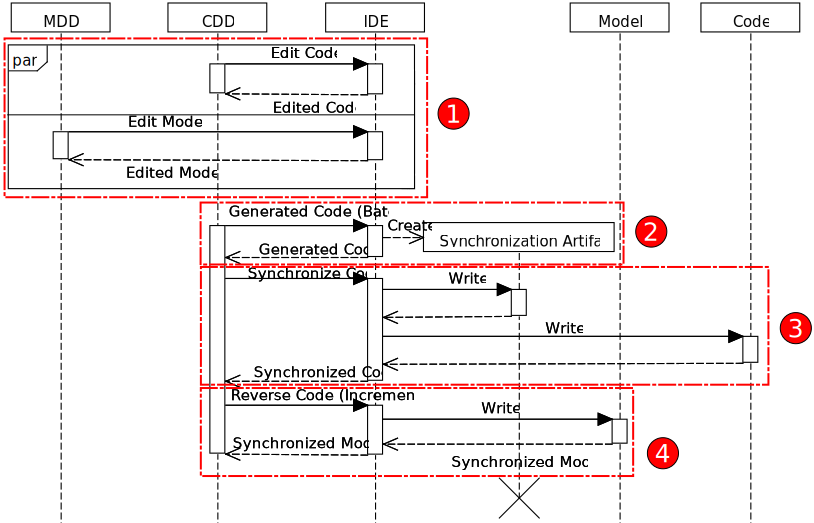
\includegraphics[width = \columnwidth]{figures/scenario3_seq}
\caption{Synchronization process, in which the model and the code are concurrently edited with code as the synchronization artifact (CDD = Code-Driven Developer, MDD = Model-Driven Developer). The API calls for Model and Code are represented generically as "Read" and "Write".}
\label{fig:scenario3}
\end{figure}

\begin{description}
	\item[Step 1] Both the model and code may be edited concurrently.
	(To simplify Figure \ref{fig:scenario3}, we don't show the Read and Write interactions for this step.)
	After both artifacts have been edited concurrently, we need to synchronize them.	
	\item[Step 2] First we create a synchronization artifact from the edited model by generating code in batch mode.
	This synchronization artifact is code and it is an image of the edited model.	
	\item[Step 3] The synchronization artifact is synchronized with the edited code. Since the synchronization artifact
is code itself, this step is done with the \texttt{Synchronize Code} use-case of the IDE.
	\item[Step 4] Once synchronization artifact and edited code are synchronized, the former is reversed incrementally to update the edited model.
\end{description}

The second strategy, based on using model as the synchronization artifact,
is the opposite of the first strategy. In the second strategy, the synchronization artifact is
obtained by reversing the edited code in batch mode.
Afterwards the synchronization artifact is synchronized with the edited model.
Finally, we generate code incrementally from the synchronization artifact to update the edited code.

%Figure \ref{fig:strategy2} shows the synchronization strategy based on using model as the synchronization artifact.
%This strategy is the opposite of the strategy presented in Figure \ref{fig:strategy1}. Its steps are described as follows:
%
%\begin{center}
%\textbf{\textit{- Steps of synchronization strategy 2 -}}
%\end{center}
%\begin{description}
%	\item[Step 1] The synchronization artifact is obtained by reversing the edited code in batch mode.
%	\item[Step 2] Afterwards the synchronization artifact is synchronized with the edited model.
%	\item[Step 3] Finally, we generate code incrementally from the synchronization artifact to update the edited code.
%\end{description}
%
%\begin{figure}
%\centering
%\includegraphics[width=\columnwidth]{figures/strategy2}
%\caption{Synchronization strategy 2 using model as synchronization artifact}
%\label{fig:strategy2}
%\end{figure}

We propose two strategies based on the preferences of the developers.
They may even use both strategies, successively, as a kind of hybrid strategy.
This may be useful
when developers want to synchronize parts of the system using one strategy,
and other parts using the other strategy. %For example, they may choose
%to synchronize method bodies using strategy 1, where the synchronization artifact is code.
%Then strategy 2, in which the synchronization artifact is a model, is used to
%to synchronize architectural elements of the system.

%In the next section we propose an implementation
%of an IDE and the proposed synchronization processes.

\section{A generic model-code synchronization pattern}
\label{sec:processes}
This section describes our generic artifact synchronization methodology pattern. 
%Although, the pattern is presented in a model-code synchronization-oriented way, it is flexibly extensible to any artifacts. 
For the sake of generality, we postulate that the architect and programmer are actors with starkly opposite development practices.
This allows the approach to be used even in cases where model
and code can both be used for the full implementation of a system,
rather than just architectural design for the former,
and code implementation for the latter.

\subsection{Definitions}
\label{sec:use-case}

In this section we define the actors who will use our model-code synchronization approach to collaborate during development.
%Then we define the main capabilities, as use-cases, expected from a generic IDE used by these actors.
Some basic concepts related to the actors and use-cases are also defined in this section.


%\subsection{Collaborating actors and development artifacts}

%In this paper we propose a methodological model-code synchronization pattern for collaboration between software
%architects and programmers.

First, we introduce the concepts of \textit{development artifact} and \textit{baseline artifact}.

\begin{definition}[Development artifact]
	A development artifact is an artifact, as defined in \cite{omg_software_2008},
	that can be used for the full implementation of the system.
\end{definition}

%For example a system can be entirely implemented as code.
%Implementation code is a development artifact, so may model.
%It is then not only documentation of specification
%but part of the implementation.
%For example a model can be used for implementation by generating code from the model, and compiling the code without the need to edit or complete the code.
In our work, we assume that model and code are both development artifacts.
A development artifact may be the baseline artifact, defined in this paper as follows:

\begin{definition}[Baseline artifact]
	A baseline artifact is one which may be edited manually.
	All other artifacts are produced from the baseline artifact
	through some process, and only through a process. Manual edition
	of artifacts other than the baseline artifact is forbidden.
\end{definition}

Two primary actors, called \textit{model-driven developer}
and \textit{code-driven developer}, are introduced.
%The main difference between them
%is what they consider as the baseline artifact.

\begin{definition}[Model-driven developer]
	A model-driven developer is an actor in a software development process
	for whom the baseline artifact is the model.
\end{definition}

%In other words, for the model-driven developer only the model should be edited manually. 
The code must always be produced from the model automatically
by some process that guarantees that the code is consistent with the model.
A software architect is a kind of the model-driven developer
who edits the model to specify the architecture of the system.
%An architect presumes that the reference for the architecture
%of the system should be specified as a model.

\begin{definition}[Code-driven developer]
	Code-driven developer is an actor in a software development process
	for whom the code is the baseline artifact.
\end{definition}

A programmer is a specialization of the code-driven developer.
Indeed, programmers may modify the code, such as editing method bodies.
%The code is then the main reference for the implementation of methods.

There are some use-cases for manual edition of artifacts. The \texttt{Edit Artifact} use-case
implies that the IDE must have some tool to let the developer manually edit an artifact.
The \texttt{Edit Model} and \texttt{Edit Code} use-cases are specializations of the \texttt{Edit Artifact}
use-case where the artifact is the model or code.

There are also some use-cases related to the synchronization of artifacts. The \texttt{Synchronize Artifact} use-case (1) compares two artifacts, (2) updates each with editions made
in the related artifact, and (3) reconciles conflicts when appropriate. The \texttt{Synchronize Model} and \texttt{Synchronize Code}
use-cases are specializations where, respectively, the model or the code are the artifacts being synchronized.

The \texttt{Generate Code} use-case is related to forward engineering.
It is the production of code in a
programming language from a model.
The developer can either use \texttt{Generate Code (Batch)} or \texttt{Generate Code (Incremental)}.
%\end{comment}

\begin{definition}[Batch code generation \cite{Giese2006}]
	Batch code generation is a process of generating code
	from a model, from scratch.
	Any existing code is overwritten by the newly generated code.
\end{definition}

Incremental code generation is a specialization of incremental model transformation, which
is defined in \cite{Giese2006} as model transformation that
does not generate the whole target model from scratch but only updates the target model by
propagating editions made in the source model.

%\texttt{Incremental code generation (ICG)} \ti{$gen_{inc}$ is a process of taking as input a changed model m and an existing executable code to make the code synchronized with the changed model: $gen_{inc}(m, c) = c'$. Non-conflicted changes at the code side are kept intact the synchronization. ICG is also defined as a process of taking model changes ch and an existing code c: $gen_{inc}(ch, c) = c'$}.

%Derived from the definition of incremental model transformation, 
Incremental code generation
is defined in this paper as follows:

\begin{definition}[Incremental code generation]
	In-cremental code generation is the process
	of taking as input an edited model, and existing code, and then updating the code by propagating
	editions in the model to the code.
\end{definition}

%\begin{comment}
Finally, the \texttt{Reverse Code} use-case is related to reverse engineering.
\texttt{Reverse Code} is the production of a model, in a modeling language, from code, written in a programming language.
The developer can either use \texttt{Reverse Code (Batch)} or \texttt{Reverse Code (Incremental)}, which are defined in this paper as follows:
%\end{comment}

\begin{definition}[Batch reverse engineering]
	Batch reverse engineering is a process of producing a model from code, from scratch.
	The existing model is overwritten by the newly produced model.
\end{definition}

\begin{definition}[Incremental reverse engineering]
	Incremental reverse engineering is the process of taking as
	input a edited code, and an existing model, and then updating the model by propagating
	editions in the code to the model.
\end{definition}

%For readability, in this paper we will sometimes designate batch and incremental as modes
%of code generation/reverse; e.g. we say that we generate code in batch mode from a model.

%The use-cases are generic. They do not depend
%on any particular approach or tool. Therefore the software developers
%can choose the approach or tool that suits better his/her
%development preferences best.

In the next section, the use-cases of the IDE are integrated into
a process that covers model-code synchronization.
%The scenarios correspond to behaviors performed by both kinds of actors,
%i.e. model-driven developers and code-driven developers.

%Model-driven engineering has been established as a potential approach to gain software quality and productivity \cite{Mussbacher2014}. 

\subsection{Processes to synchronizing model and code}

We propose two synchronization strategies for this scenario.
The general approach behind our strategies
is to represent one artifact in the language of its corresponding other artifact.
These two can then be compared. For this, we define a
concept of a \textit{synchronization artifact}:

\begin{definition}[Synchronization artifact]
An artifact used to synchronize a model and its corresponding code
is called a synchronization artifact.
It is an image of one of the artifacts, either the model or the code.
In this context, an image $I$ of an artifact $A$ is a copy of $A$ obtained by
transforming $A$ to $I$. $A$ and $I$ are semantically equivalent but are specified in different languages.
\end{definition}

For example, a synchronization artifact can be code that was generated from the edited model in batch mode.
In that case, it is code that represents an image of the edited model (being image requires that the model is able to be reconstructed from the code).

Using the concept of synchronization artifact, two strategies are
proposed in this paper: one in which the synchronization artifact is code,
and the other in which the synchronization artifact is a model.
The developer can choose to either use these two use-cases of the IDE. The choice may be determined by
preferred development practices or the availability of suitable tools (e.g. the programmer
may prefer to synchronize two artifacts, both represented
in the same programming language, because he prefers to
work exclusively with code).

Figure \ref{fig:scenario3} shows the first synchronization
strategy based on using code as the synchronization artifact.
The general steps of the process shown in Figure \ref{fig:scenario3} are described as follows:

\begin{figure}
\centering
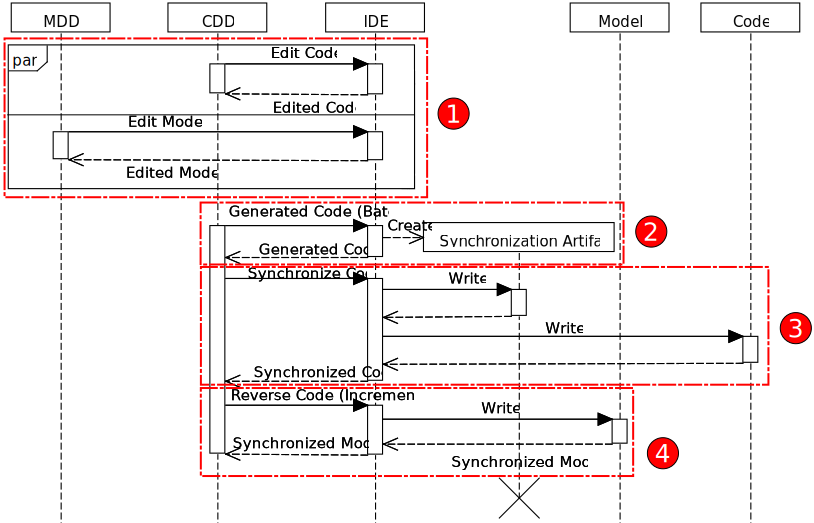
\includegraphics[width = \columnwidth]{figures/scenario3_seq}
\caption{Synchronization process, in which the model and the code are concurrently edited with code as the synchronization artifact (CDD = Code-Driven Developer, MDD = Model-Driven Developer). The API calls for Model and Code are represented generically as "Read" and "Write".}
\label{fig:scenario3}
\end{figure}

\begin{description}
	\item[Step 1] Both the model and code may be edited concurrently.
	(To simplify Figure \ref{fig:scenario3}, we don't show the Read and Write interactions for this step.)
	After both artifacts have been edited concurrently, we need to synchronize them.	
	\item[Step 2] First we create a synchronization artifact from the edited model by generating code in batch mode.
	This synchronization artifact is code and it is an image of the edited model.	
	\item[Step 3] The synchronization artifact is synchronized with the edited code. Since the synchronization artifact
is code itself, this step is done with the \texttt{Synchronize Code} use-case of the IDE.
	\item[Step 4] Once synchronization artifact and edited code are synchronized, the former is reversed incrementally to update the edited model.
\end{description}

The second strategy, based on using model as the synchronization artifact,
is the opposite of the first strategy. In the second strategy, the synchronization artifact is
obtained by reversing the edited code in batch mode.
Afterwards the synchronization artifact is synchronized with the edited model.
Finally, we generate code incrementally from the synchronization artifact to update the edited code.

%Figure \ref{fig:strategy2} shows the synchronization strategy based on using model as the synchronization artifact.
%This strategy is the opposite of the strategy presented in Figure \ref{fig:strategy1}. Its steps are described as follows:
%
%\begin{center}
%\textbf{\textit{- Steps of synchronization strategy 2 -}}
%\end{center}
%\begin{description}
%	\item[Step 1] The synchronization artifact is obtained by reversing the edited code in batch mode.
%	\item[Step 2] Afterwards the synchronization artifact is synchronized with the edited model.
%	\item[Step 3] Finally, we generate code incrementally from the synchronization artifact to update the edited code.
%\end{description}
%
%\begin{figure}
%\centering
%\includegraphics[width=\columnwidth]{figures/strategy2}
%\caption{Synchronization strategy 2 using model as synchronization artifact}
%\label{fig:strategy2}
%\end{figure}

We propose two strategies based on the preferences of the developers.
They may even use both strategies, successively, as a kind of hybrid strategy.
This may be useful
when developers want to synchronize parts of the system using one strategy,
and other parts using the other strategy. %For example, they may choose
%to synchronize method bodies using strategy 1, where the synchronization artifact is code.
%Then strategy 2, in which the synchronization artifact is a model, is used to
%to synchronize architectural elements of the system.

%In the next section we propose an implementation
%of an IDE and the proposed synchronization processes.

\section{An Implementation: synchronizing UML models and C++ code}
\label{sec:implementation}

The proposed model-code synchronization approach can be automated.
We examine an Eclipse-based implementation of the IDE proposed in
Section \ref{sec:use-cases_ide}. The implementation is used in the synchronization processes
proposed in Section \ref{sec:processes}.
Our implementation targets synchronization of Object Management Group (OMG) standard UML 2 and C++11 code.

The use-cases of the IDE are implemented with some Eclipse technologies. More information
on the technologies is available on the Eclipse Projects website \cite{eclipse_foundation_eclipse_2016}.

\textbf{Eclipse CDT} is an IDE for C++ development. It is used in the \texttt{Edit Code} use-case.
Eclipse \textbf{Papyrus} is used for the \texttt{Edit Model} use-case.
Papyrus is an open-source UML modeler that uses the Eclipse Modeling Framework (EMF)
implementation of the OMG-standard UML 2.
Papyrus supports UML profiles for domain-specific modeling, and we use the UML profile of Papyrus
dedicated to C++ to facilitate and accelerate modeling of some C++ features.
%Furthermore, in standard UML there are elements like OpaqueBehavior which
%allow to express programming language specifics in the model.

We developed plugins for Papyrus to \texttt{Generate Code} from UML to C++ and to \texttt{Reverse Code}.
The batch modes of these use-cases do not need additional technologies to implement.
For use-cases \texttt{Generate Code (Incremental)} and \texttt{Reverse Code (Incremental)}, we choose to
listen to modification events in the model and code respectively. Listening to modification events
is one possible approach in incremental model transformation \cite{kusel_survey_2013}.
The \textbf{Viatra}
API is used to listen to such events in the model. The Eclipse CDT API is used
to listen to modification events in the code. These list of events are used to
either generate code or reverse code incrementally.

\textbf{EMF Compare} is used for the \texttt{Synchronize Model} use-case when
models are implemented with EMF.
We adapted EMF Compare in order to synchronize UML models for
our specific work.
Eclipse CDT is used for the \texttt{Synchronize Code} use-case with its built-in C++ features.



%Figure \ref{fig:strategies_impl} shows how technologies are combined
%for UML-C++ synchronization, within a same Eclipse IDE. The synchronization strategies,
%in the scenario where model and code are concurrently edition, is taken as an example to
%show how the technologies are involved in the synchronization processes.
%
%\begin{figure}
%\centering
%\includegraphics[width=\columnwidth]{figures/strategies_impl}
%\caption{Implementation of synchronization strategies}
%\label{fig:strategies_impl}
%\end{figure}

The next section describes some experiments performed using the above implementation
of our synchronization solution.
\section{Experiments and Evaluations}
\label{sec:experiments}

This section reports our experiments with the proposed model-code synchronization approach
and its implementation
based on Eclipse technologies.
The contributions are applied for UML and C++.
Two experiments have been conducted in order to assess the proposed methodology and
its applicability to the development of a realistic system.
In the following subsections, we first describe the results of some simulations designed
to test the proposed approach. Next, we report on a realistic case-study intended to help us assess certain scalability and usability aspects.

\subsection{Simulations to assess synchronization processes}
\label{sec:simulation}

Simulations have been conducted to test that the implementation of
our proposition respects the round-trip engineering
laws \cite{Foster:2007:CBT:1232420.1232424}
\ti{right-invertibility} and \ti{left-invertibility}.
These laws are stated as follows:

%The RTE takes as input the previous consistent model and code and their edited versions and outputs the updated artifacts: \ti{rte(m, c, m*, c*) = ($m_{updated}, c_{updated}$)}. A round-trip must satisfy two laws, namely, \ti{right-invertibility} and \ti{left-invertibility} stated as followings:

\noindent
\tb{Law 1}: Right-invertibility means that
not editing the code (or model, respectively) shall be reflected
as not editing the model (respectively code).
If no editions are made to the code, the model used for generating the code and the model received by
immediately reversing the generated code must be the same.

\noindent
\tb{Law 2}: Left-invertibility means that all editions
on the code are captured and correctly
propagated to the model
so that the edited code can be fully recreated by applying code generation to the updated model.

In the following sections, the model generator used for the simulations is
presented first. Then, the simulations performed for both above laws are described.
Finally, we discuss the simulation of the process defined for scenario 3 (Section \ref{sec:scenario3}), in which both the model and the code are edited concurrently.

\subsubsection{Randomly generated UML models}

In the simulations, random UML models are generated
with a configurable model generator.
The generated models contain C++ features represented via UML.
The generator can be configured to generate a desired average number of each type of C++ feature to be represented as a UML element.

Three packages are generated for each model.
Each package contains 60 classes, and, on the average
10 enumerations, 10 structures, and
10 function pointers. Class members include
methods with parameters, and attributes.

Types of parameters and attributes are chosen randomly.
Methods have randomly generated bodies that use other classes.
Attributes have randomly generated default values of the appropriate types.

Relationships between
classes are also generated: associations, inheritances, and dependencies.
When dependencies are generated, the generator enforces that the source
class of the dependency has a method that uses the target class of the dependency.

%Some parameters of the model generator are shown in Table \ref{table:info-setup}.
%
%% TODO I don't know if the table itself is useful.
%\begin{table}[]
%\centering
%\caption{Appearance probabilities and information for setting up the model generator}
%\label{table:info-setup}
%\begin{tabular}{|l|l|}
%\hline
%\rowcolor{Gray}
%Generator configuration                                   & Value            \\ \hline
%Number of packages                                        & 3 \\ \hline
%Number of classes per package                             & 60              \\ \hline
%Number of attributes per class                            & 30               \\ \hline
%Attribute appearance probability                          & 0.5              \\ \hline
%Probability of having an attribute default value          & 0.3              \\ \hline
%Number of methods per class                               & 15               \\ \hline
%Probability of appearance for a method                    & 0.5              \\ \hline
%Number of parameters per operation                        & 4                \\ \hline
%Probability of appearance for a parameter                 & 0.5              \\  \hline
%Maximum number of generalizations                         & 300              \\ \hline
%Number of data types per package                          & 10               \\ \hline
%Probability of appearance for a structure                 & 0.3              \\ \hline
%Number of enumerations per package                        & 10               \\ \hline
%Probability of appearance for an enumeration              & 0.3              \\ \hline
%Number of function pointers per package                   & 10               \\ \hline
%Probability of appearance for a function pointer          & 0.3              \\ \hline
%\end{tabular}
%\end{table}

\subsubsection{Simulation for Law 1 right-invertibility}

In the first simulation, Law 1 is evaluated. The procedure for the simulation is shown
in Figure \ref{fig:simulation1}.

\begin{figure}
\centering
\includegraphics[width=\columnwidth]{figures/simulation1}
\caption{Simulation 1 for Law 1 (right-invertibility)} 
\label{fig:simulation1}
\end{figure}

The general idea behind the simulation procedure is to
do a full round-trip of the UML model randomly generated in step \textbf{(1)}.
The round-trip of the model is done through steps \textbf{(2)} to \textbf{(3)}.
The randomly generated model is compared with the reversed model after the round-trip. This is done in step \textbf{(5)}.

A full round-trip is also done for the C++ code that is generated
from the original randomly generated model in step \textbf{(2)}.
The round-trip is done through steps \textbf{(3)} to \textbf{(4)}. 
The code generated from the original
model is compared with code generated from the reversed model
in step \textbf{(6)}.

Code generation and reverse are done in batch mode since
no editions are made to the models or code in this simulation.
Comparison of models is done by first comparing the number of each type of elements. If these numbers match, EMF Compare is used.
Comparison of code is done by using the built-in code comparison tool in the Eclipse CDT.

Table \ref{tab:generated_models} shows the number of each type of elements in the randomly
generated model,
and the comparison results, for 3 of the 200 models created by the generator.
We limited ourselves to 200 models for practical reasons.
These same models were later used for a simulation that involved some manual editions (presented
in the next subsection).

After launching the simulation for the 200 models, no differences
were found during model comparison and code comparison.
This result assesses that the tooling of our model-code synchronization approach
with respect to Law 1 of round-trip engineering.

\begin{table*}[]
\centering
\caption{Three of 200 generated models for simulation 1: Abbreviations are classes (\tb{C}), methods (\tb{M}), method parameters (\tb{P}), attributes (A), associations (\tb{AS}), inheritances (\tb{G}), method body (\tb{B}), dependencies (\tb{D}), enumerations (\tb{E}), structures (\tb{S}), default values (\tb{DV}), function pointers (\tb{F})}
\label{tab:generated_models}
\begin{tabular}{|l|l|l|l|l|l|l|l|l|l|l|l|l|p{4pc}|p{4pc}|}
\hline
\rowcolor{Gray}
Model ID & C   & M    & P    & A    & AS   & G   & B    & D   & E  & S & DV  & F  & Differences in models? & Differences in code?\\ \hline
1        & 180 & 1419 & 2683 & 1835 & 1053 & 179 & 1138 & 507 & 13 & 7 & 150 & 11 & No & No\\ \hline
2        & 180 & 1437 & 2718 & 1874 & 1074 & 179 & 1157 & 512 & 10 & 9 & 167 & 9  & No & No\\ \hline
..       & ..  & ..   & ..   & ..   & ..   & ..   & ..  & .. & ..& ..  & ..  & .. & No & No\\ \hline
200      & 180 & 1413 & 2629 & 1857 & 1018 & 179 & 1127 & 517 & 13 & 9 & 150 & 13 & No & No\\ \hline
\end{tabular}
\end{table*}

\subsubsection{Simulation for Law 2 left-invertibility}
\label{sec:simulation2}

In the second simulation, Law 2 was evaluated. The procedure for the simulation is shown
in Figure \ref{fig:simulation2}.

\begin{figure}
\centering
\includegraphics[width=\columnwidth]{figures/simulation2}
\caption{Simulation 2 for Law 2 (left-invertibility)} 
\label{fig:simulation2}
\end{figure}

The general idea behind the simulation procedure is to
do a full round-trip of a randomly generated UML model,
but with editions introduced to the generated C++ code.
As shown in Figure \ref{fig:simulation2}, the
procedure to test our tooling consisted of the following steps:

\begin{description}
	\item[Step 1] A UML model is randomly generated and becomes the \textbf{generated model}.
	\item[Step 2] Through batch code generation, we obtain \textbf{code from generated model}.
	\item[Step 3] The code produced from generated model is then edited.
	We thus obtain \textbf{edited code}.
	The different kinds of editions will be described
	when we discuss the results of this simulation.
	\item[Step 4] The \textbf{edited code} is reversed incrementally to the \textbf{generated model}.
	The \textbf{generated model} then becomes an \textbf{updated model}.
	\item[Step 5] The \textbf{edited code} is also reversed in batch mode
	to a \textbf{model from edited code}.
	This model is an image of the edited code.
	\item[Step 6] The \textbf{updated model} (the previously \textbf{generated model})
	is compared to the \textbf{model from edited code} (image of the edited code).
	\item[Step 7] Afterwards, we also generate in batch mode \textbf{code from the updated model}.
	\item[Step 8] The \textbf{code from the updated model} is compared to the \textbf{edited code}.
\end{description}

The simulation is run for 200 randomly generated models.
We limited ourselves to 200 models because in step \textbf{(3)}, some of the editions
have to be done manually to emulate real development conditions.
Therefore the limit of 200 models is purely based on practical concerns.

During the simulations, the code generated from each model undergoes seven kinds of
editions independently (the kinds of editions performed are listed in Table \ref{tab:change_description}).
As its name suggests, only "Manual editions" were done manually by a developer, to emulate
actual development conditions.

The editions triggered three kinds of Eclipse CDT modification events:
\texttt{ADDED}, \texttt{REMOVED}, and \texttt{CHANGED}. Events \texttt{ADDED} and \texttt{REMOVED}
mean addition and deletion
of classes, attributes or methods to the code.
Event \texttt{CHANGED} is the update of elements in code including
(1) renaming attributes, classes, or methods, (2) changing the
type of attributes, parameters, or (3) changing the behavior of methods.

Table \ref{tab:change_description} shows the average number of \texttt{ADDED}, \texttt{REMOVED}, and \texttt{CHANGED} events
that were triggered by each of the seven kinds of editions. The last two columns
show the results of model comparison and code comparison for all 200 simulations following
each kind of edition (the editions are made independently).

\begin{table}[]
\centering
\caption{Editions and the modifications events they trigger (A = \texttt{ADDED}, C = \texttt{CHANGED}, R = \texttt{REMOVED})}
\label{tab:change_description}
\begin{tabular}{|p{2cm}|l|l|l|l|l|}
\hline
\rowcolor{Gray}
Edition kind                                              & A   & C    & R   & \begin{tabular}[c]{@{}l@{}}Model\\diff?\end{tabular} & \begin{tabular}[c]{@{}l@{}}Code\\diff?\end{tabular} \\ \hline
Renaming attributes of all classes                             &  0  & 1903 &  0   & \multicolumn{1}{c|}{No} & \multicolumn{1}{c|}{No} \\ \hline
Renaming methods of all classes                                &  0  & 1197 &  0   & \multicolumn{1}{c|}{No} & \multicolumn{1}{c|}{No} \\ \hline
Deleting attributes                                            &  0  &    0 & 46   & \multicolumn{1}{c|}{No} & \multicolumn{1}{c|}{No} \\ \hline
Adding attributes                                              & 25  &    0 &  0   & \multicolumn{1}{c|}{No} & \multicolumn{1}{c|}{No} \\ \hline
Adding methods                                                 & 10  &    0 &  0   & \multicolumn{1}{c|}{No} & \multicolumn{1}{c|}{No} \\ \hline
Changing method body                                           &  0  & 30   &  0   & \multicolumn{1}{c|}{No} & \multicolumn{1}{c|}{No} \\ \hline
Manual editions                                           & 39  & 34 & 30   & \multicolumn{1}{c|}{No} & \multicolumn{1}{c|}{No} \\ \hline
\end{tabular}
\end{table}

For all 200 models, no differences
were found during model comparison and code comparison.
This result assesses that the tooling of our model-code synchronization approach
with respect to Law 2 of round-trip engineering.

\subsubsection{Simulation for concurrent edition of model and code}

A third simulation aims at emulating the process described in Figure \ref{fig:scenario3} of Section \ref{sec:scenario3},
in which the model and the code are concurrently edited.
A simplified representation of the procedure of simulation 3 is shown in Figure \ref{fig:simulation3}.
The simulation is executed for 200 randomly generated
UML models and their generated C++ code.

\begin{figure}
\centering
\includegraphics[width=6.5cm]{figures/simulation3}
\caption{Simulation 3 for concurrent editions case}
\label{fig:simulation3}
\end{figure}

The idea behind the procedure in Figure \ref{fig:simulation3} is to simulate editions in the original randomly generated model,
and its corresponding generated code (step \textbf{(1)} to \textbf{(4)}).
To simplify the simulation, the simulator only introduces attribute renaming model-side.
On the code-side, the simulator only makes editions to method bodies.
Edited model and code must then be synchronized and then we must assess that they are
indeed synchronized. This is done in step \textbf{(5)}.

To synchronize edited model
and edited code, first we use the strategy based on code as the synchronization artifact. 
The simulator propagates all method body editions from the edited code to the synchronization
artifact. The simulator then propagates all attribute renaming from the synchronization
artifact to the edited code. Next, the synchronization artifact is reversed incrementally to
produce the edited model. At this point the model and the code are considered synchronized.

To assess that both synchronized model and code are images of one another, the synchronized code was
reversed in batch mode to a new model. The new model was then compared with the synchronized model. No
differences were found during these simulations. We also generated new code in batch mode
from the synchronized model. The new code was compared to the synchronized code. No differences
were found during the comparison.

The same simulation is repeated for the case where the model is used as synchronization
artifact. Again the synchronized code and model were images of one another.
%Therefore with this example of concurrent edition of model and code,
%our proposition is tested.

Once the tooling of the proposed model-code synchronization approach
was verified through the three simulations,
we decided to apply it to the development of a practical real-world system.
The results of this experiment are discussed in the next section.

\subsection{Papyrus-RT runtime case-study}
\label{sec:case-study}

% Section introduction and goal of experiment
In Section \ref{sec:simulation} the approach was tested for UML and C++ synchronization, using simulations.
In this section we describe the application of the full synchronization approach to a case-study. The intent here was to evaluate:

\begin{itemize}
	\item The usability of the proposed synchronization approach
	\item The scalability of the tooling to a real system
\end{itemize}

% Case-study introduction
The case-study is related to the development of the runtime underlying Papyrus-RT \cite{cea_papyrus-rt_2016}.
This latter is an open-source custom modeling tool, based on Papyrus,
that supports UML extensions for the design of a category of event-driven real-time systems (UML-RT).
%UML-RT \cite{kuster_consistent_2001} offers
%a set of extensions to UML for the design of real-time systems. UML-RT is
%developed by Zeligsoft within the Papyrus-RT \cite{cea_papyrus-rt_2016} modeler dedicated to the UML-RT modeling language.
Papyrus-RT features full automated code generation for UML
models. 
The generated code executes within a corresponding runtime environment,
which provides C++ realizations of the high-level concepts defined in UML-RT.

% Motivation behind case-study
At the beginning of the project,
the resource available to develop the aforementioned runtime
was an experienced C++ programmer.
For the obvious pragmatic reasons of project management,
it was decided to implement the runtime in C++ without
the benefits of models.
However, later it was concluded that even if the result was satisfactory,
it would be beneficial to exploit the advantages that MDE provides.
Thus, an MDE approach would improve
both the maintainability and the evolvability of the runtime.
Moreover, as development progressed, the project was expanded to include
new developers, who are proponents
of MDE and are eager to work with models.

As a result, this project represented an ideal case study to assess the practicality of the proposed approach. In particular, we were interested in determining its usability and scalability

% C++ implementation and C/C++ specificities of case-study
The runtime was originally implemented as an open-source plain C++11 project.
Most of its architecture is object-oriented.
The runtime has 65 classes and 14,945 lines of code.
Other than containing typical entities found in object-oriented architectures,
the runtime uses C/C++ features such
as type definitions, templates, pointers, references, function pointers, and variadic functions to name a few.
These features are supported by the
the reverse and code generation tools in Papyrus, coupled with the C++ UML profile.

% What we did in the experiment
In order to use our model-code synchronization approach, the original Papyrus-RT runtime had first to be
reversed to a UML model. This step was crucial because the original runtime
contained some elements that were not object-oriented. Consequently,
some modifications and refactorings were made
to the original runtime to make it fully object-oriented.
This enabled it to be modeled entirely in a language like UML.
Table \ref{tab:runtime_diff} shows the two main differences between
the original runtime, and the revised object-oriented runtime.

\begin{table}
\centering
\caption{Differences in Papyrus-RT runtime versions}
\label{tab:runtime_diff}
    \begin{tabular}{|p{9pc}|p{9pc}|}
    \hline
    \rowcolor{Gray}
    Original & Object-oriented \\ \hline
    Directives to control compilation of OS-dependent code & Abstract OS-independent classes inherited by OS-dependent classes with implementation \\ \hline
    Variables, functions and type definitions outside of class & Refactored as entities inside a class. Attributes and functions are static with visibility defined according to scope of original variables and functions. \\ \hline
    \end{tabular}
\end{table}

% Results
The reverse in batch mode of the object-oriented runtime
takes about 12 seconds. All 65 classes were reversed,
with all of their attributes and methods.
Code generation in batch mode of the entire reversed UML model takes about 5 seconds
and produces 22,053 lines of code.
The difference in the number of lines of code is due to automatically
generated documentation comments.
The generated runtime compiles and the updated existing unit tests
pass when applied on the runtime compiled from generated code.

Once the runtime has been reversed,
our model-code synchronization processes could be used.
We noticed that using the proposed approach introduced MDE style development for the Papyrus-RT runtime.
This brought about several advantages as several manual tasks were automated:

\begin{itemize}
	\item Automatic handling of relationships between model elements, i.e. association, dependency, inheritance
	\item Automatic generation of includes and forward declarations in the code that avoids cyclic dependencies
	\item Graphical representation of architecture in automatically updated UML diagrams (feature of Papyrus)
\end{itemize}

In applying the proposed approach to achieve a collaborative development of the runtime system,
we found that the only real difficulty faced was initializing the synchronization processes.
This required the reverse engineering of the original runtime, with some non-object-oriented code, into an
object-oriented UML model. The reverse was successful following some modifications and refactorings.
Once the full model-code synchronization process was in place,
we were able to use it and develop concurrently both the UML model and its generated C++ code.
%The development of the runtime then benefited from automation through MDE.


In the following section we relate both our work, including the implementation, to
existing approaches and tools presented in the literature.
\section{Conclusion}
\label{sec:conclusion}

Model-Driven Engineering is considered an efficient way to dealing with the complexity of systems today. 
MDE relies on two mechanisms abstraction and automation. 
The latter are realized by artifact synchronizations.  
Despite many advantages of MDE, the adoption level of MDE into industries is still not high as expected. 
In order to raise the adoption level, the core technologies of MDE need to be enhanced.   
This report presents the scope of the thesis, whose focus is to improve the core technologies of MDE such as artifact transformation, synchronization and code generation. 

The report starts with describing major topics covered and developed in the deployment of the thesis. 
Different approaches around the technologies are proposed for wider integrating MDE into industrial practice to gain software quality and productivity. The proposed approaches are designed to support a continuous collaboration between software architects and programmers allowing each to use the working practices of choice
%It can be used as a pattern
%to solve the issue of model-code synchronization when artifacts co-evolve.
%The proposition targets collaboration between software architects and programmers,
%without imposing to either developers a diagram-based language or a textual language.

Two approaches including a generic pattern for artifact synchronization and a complete generation solution for UML State Machine are chosen to be detailed in this report because of their importance. 
Other works are also mentioned in the report. 
The overview of some ongoing and future works is also described to provide readers a plan for the next steps of the thesis deployment.  

\begin{comment}
Several simulations were used to validate our synchronization approach with respect to both laws of round-trip engineering. 
In addition, a simulation of scenarios in which both the model and the code were edited concurrently was performed, further demonstrating the viability of the approach, even in such a highly dynamic scenario.

The approach was then applied to a real-world application: the Papyrus-RT runtime system. This system was
originally developed in C++ with some non-object-oriented code.
The experiment showed that the main difficulty of using our approach applied to such a system was
the need to edit and refactor the program code in such way that it can be reverse engineered into a corresponding UML model without loss of information.
Once the processes of our synchronization solution were bootstrapped in this way, dynamic collaboration
between software architects and programmers was possible. We were then able to
reap the important benefits of MDE; development was facilitated through increased automation and system maintainability and evolvability were improved.

%Realization-wise, in the future, we would like to make our implementation even more generic.
%Indeed, we had to modify tools like EMF Compare to suit the
%implementation of our solution with other Eclipse technologies.
Currently we are implementing our generic synchronization pattern for several other
programming languages, like Java. Part of our future work is to federate
implementations of the system, in heterogeneous programming languages,
as one or several models based on a common core in UML.
\end{comment}
%The work presented in this report is supported by the European project SafeAdapt, grant agreement No. 608945, see \ti{http://www.SafeAdapt.eu}. The project deals with adaptive system with additional safety and real time constraints. The adaptation and safety aspects are stored in different artifacts in order to achieve a separation of concerns. These artifacts need to be synchronized. In this project in part motivated by the perceived gap between diagram-based languages and
%textual languages, which impeded greater adoption of MDE among practitioners.

%Therefore, as a future work item, we would like to assess to what extent our
%solution helps in eliminating the unnecessary and dogmatic separation of models from code. 
%We feel that this would be useful to both the MDE community and the more traditionally-oriented software communities.
%As MDE is gradually integrated into industrial practices, correct-by-construction approaches, through MDE,
%can be adopted to deliver higher quality software.

%\input{sections/ack}
\bibliographystyle{abbrv}
\bibliography{refs}

\end{document}
